%%%%%%%%%%%%%%%%%%%%%%%%%%%%%%%%%%%%%%%%%%%%%%%%%%%%%%%%%%%%%%%%%%%%%%%%%%%%%%%
%                                                                             %
% Anwendungsbeispiel für das Beamer-Template TU Chemnitz                      %
% (c) Mario Haustein (mario.haustein@hrz.tu-chemnitz.de), 2013-2014           %
%                                                                             %
%%%%%%%%%%%%%%%%%%%%%%%%%%%%%%%%%%%%%%%%%%%%%%%%%%%%%%%%%%%%%%%%%%%%%%%%%%%%%%%

\usepackage{ifxetex}
\usepackage{ifluatex}
\ifxetex
\usepackage[babelshorthands]{polyglossia}
\setmainlanguage{german}
\else\ifluatex
\usepackage[babelshorthands]{polyglossia}
\setmainlanguage{german}
\else
\usepackage[utf8]{inputenc}
\usepackage[ngerman]{babel}
\fi\fi
\usepackage{url}
\usepackage{tikz}
\usepackage{amsmath}
\usepackage{exscale}
\usepackage{listings}
\usepackage{listingsutf8}
\usepackage{textcomp}
\usepackage{chemfig}
\usepackage{metalogo}
\usepackage{tabularx}



% Trennstellen für URLs
\def\UrlBreaks{\do\:\do\.\do\@\do\\\do\/\do\!\do\_\do\|\do\;\do\>\do\]%
 \do\)\do\,\do\?\do\'\do+\do\=\do\#}
\def\UrlBigBreaks{}

% Voreinstellungen für Quellcodelistings
\lstset{basicstyle=\ttfamily,keywordstyle=\fontfamily{lmss}\bfseries,breaklines,tabsize=2}
\ifxetex\else\ifluatex\else\lstset{inputencoding=utf8/latin1}\fi\fi
\lstdefinestyle{block}{basicstyle=\ttfamily,keywordstyle=\fontfamily{lmss}\bfseries,breakindent=10pt}
\lstdefinestyle{numberedblock}{basicstyle=\ttfamily,keywordstyle=\fontfamily{lmss}\bfseries,numbers=left,numberstyle=\scriptsize,xleftmargin=20pt,frame=leftline,breakindent=10pt}

% TUC-Templates laden.
\usetheme{tuc2014}
\mode<article>{\usepackage{beamerarticletuc2014}}


% Metadaten
\title{\LaTeX-Beamer an der TU Chemnitz}
\subtitle[Anleitung und Musterbeispiel]{Anleitung und Musterbeispiel für das \texttt{tuc2014}-Beamer-Template}
\author{Mario Haustein}
\date[\today]{Stand: \today}
\institute[TUC, URZ]{TU Chemnitz, Universitätsrechenzentrum}
\titlegraphic{
\includegraphics[height=0.2\textheight]{tuc2014/logo/tuc_green}}
\tucurl{http://www.tu-chemnitz.de/urz/}


\begin{document}
\begingroup
\tucthreeheadlines
\frame{\titlepage}
\endgroup

\begin{frame}
\frametitle{Die \LaTeX-Beamer-Vorlage für die TU Chemnitz}

\begin{itemize}
\item Diese Vorlage besteht aus folgenden Komponenten:
  \begin{description}
  \item[\texttt{doku.pdf}]  Dieses Dokument; Anleitung und Beispielsammlung für
                            diese Vorlage bzw. \LaTeX-Beamer allgemein.
  \item[\texttt{demo/}]     Die \LaTeX-Quellen für \texttt{doku.pdf}
  \item[\texttt{ready2go/}] Eine Vorlage, die ohne Installation verwendet werden kann.
  \item[\texttt{tds/}]      Installationsdateien
  \end{description}

\bigskip

\item Systemweite Installation
  \begin{itemize}
  \item Kopieren Sie den Inhalt des Verz. \texttt{tds/} in ihren
        \TeX-Verzeichnisbaum (z.B. \texttt{/usr/local/share/texmf/} oder
        \texttt{\textasciitilde/texmf/}).
  \item Führen Sie \texttt{texmf} bzw. \texttt{texhash} aus, um den Cache zu
        aktualisieren.
  \item Alle \texttt{.sty}-Dateien und das Verz. \texttt{tuc2014} in der
        Vorlage werden nun nicht mehr benötigt und können gelöscht werden.
  \end{itemize}
\end{itemize}
\end{frame}


\frame{\frametitle{Gliederung}\tableofcontents}
\note{\begin{itemize}
\item Weitere Anmerkungen \dots
\item \dots\ in Stichpunkten \dots
\item \dots\ formuliert.
\end{itemize}}

\section{Anwendungsbeispiele für \LaTeX-Beamer}
\subsection{Formatierung}
\begin{frame}
\frametitle{Titel}
\framesubtitle{Subtitel}
\par Das hier ist \textbf{fett}.
\par Das hier ist \textsl{schräg}.
\par Das hier ist \textit{kursiv}.
\par Das hier sind \textsc{Kapitälchen}.
\par Das hier sind \textrm{Serifen}.
\par Das hier ist \texttt{dicktengleich}.
\par Das hier ist \structure{wichtig}.
\par Das hier ist \alert{noch wichtiger}.
\par Fuß\footnote{noten}
\end{frame}


\begin{frame}
\frametitle{Blöcke}

\begin{block}{\vphantom{X}\smash{Block}}
Inhalt
\end{block}

\medskip

\begin{alertblock}{\vphantom{X}\smash{Achtung}}
Vorsicht
\end{alertblock}

\medskip

\begin{exampleblock}{\vphantom{X}\smash{Beispiel}}
\(1 + 1 = 2\)
\end{exampleblock}
\end{frame}

\begin{frame}
\frametitle{Spalten}

\begin{columns}
\begin{column}{0.6\textwidth}
Spalte 1
\end{column}
\begin{column}{0.3\textwidth}
Spalte 2
\end{column}
\end{columns}
\end{frame}


\subsection{Listen}
\begin{frame}
\frametitle{Listen}

\begin{itemize}
\item Punkt 1
\item Punkt 2
\end{itemize}

\begin{enumerate}
\item Punkt 3
\item Punkt 4
\end{enumerate}

\begin{description}
\item[Punkt] 5
\item[Punkt] 6
\end{description}
\end{frame}


\subsection{Mathematik}
\begin{frame}
\frametitle{Höhere Mathematik}

Pythagoras: \(a^2 + b^2 = c^2\), Einstein: \(E = mc^2\)

\[\nabla \times \vec{H} = \vec{j}_l + \dfrac{\partial\vec{D}}{\partial t} \quad\Longleftrightarrow\quad
\oint_{\partial A} \vec{H} \cdot \mathrm{d\vec{s}} = \iint_{A} \vec{j}_l \cdot \mathrm{d}\vec{A} +
\left(\iint_{A} \dfrac{\partial\vec{D}}{\partial t} \cdot \mathrm{d}\vec{A}\right)\]

\begin{Satz}[Cook, 1971]
\centering SAT ist \(\mathcal{NP}\)-vollständig.
\end{Satz}
\end{frame}


\subsection{Bilder}
\begin{frame}
\frametitle{Abbildungen}

\begin{columns}
\begin{column}{0.47\textwidth}
\begin{figure}
\chemfig{H-[2]C(<[:170]H)(<:[:120]H)-[:20]C(-[2]H)(<:[:-20]OH)<[:-70]H}
\caption{Prost!}
\end{figure}
\end{column}
\begin{column}{0.47\textwidth}
\begin{figure}
\chemfig{H-[:52]O-[:-52]H}
\caption{Dihydrogenmonoxid}
\end{figure}
\end{column}
\end{columns}
\end{frame}


\subsection{Quellcode}
\begin{frame}[containsverbatim]
\frametitle{Quellcode}

\begingroup
\small
\begin{lstlisting}[style=numberedblock,language=C]
#include <stdio.h>

int main(int argc, char **argv)
{
  int x = 2;

  x = x * (x + 1);
  x = 7 * x;
  printf("Die Antwort lautet: %d\n", x);

  return x;
}
\end{lstlisting}
\endgroup
\end{frame}



\section{Das Template}
\begin{frame}[containsverbatim]
\frametitle{Beamer-Themes für das TUC2014-Layout}

\begin{itemize}
\item Für das TUC-Layout wurde ein eigenes Beamer-Theme erstellt.
\item Es kann über \lstinline[language={[LaTeX]TeX}]+\usetheme{tuc2014}+ geladen werden.
\item Dadurch werden wiederum folgende Unter-Themes geladen:
  \begin{description}
  \item[Color Theme] Legt das Farbschema für jeder Fakultät fest.
  \item[Font Theme]  Lädt die Hausschrift "`Roboto Condensed"'.
  \item[Inner Theme] Legt dir Formatierung von Hervorhebungen, Aufzählungslisten,
                     Titelseite und Inhaltsverzeichnis fest.
  \item[Outer Theme] Stellt die Formatierung von Kopf- und Fußzeile sowie der
                     linken Logospalte einer Folie ein.
  \end{description}

\bigskip

\item Die Teil-Themes können ggf. auch unabhängig voneinander genutzt werden.
  \begin{itemize}
  \item In den meisten Fällen wird es aber nur Sinn machen das Color Theme
        und/oder das Font Theme im Kombination mit anderen Beamer-Themes zu
        nutzen.
  \end{itemize}
\end{itemize}
\end{frame}


\begin{frame}[containsverbatim]
\frametitle{Zusatzfunktionen des Haupt-Themes}

\begin{itemize}
\item Folgende Einstellungen werden Haupt-Theme \structure{zusätzlich} zum
      Laden der Unter-Themes vorgenommen.
  \begin{itemize}
  \item \lstinline[language={[LaTeX]TeX}]+\usefonttheme{professionalfonts}+ \\
        für die üblichen Mathematik-Schriften
  \smallskip
  \item \lstinline[language={[LaTeX]TeX}]+\setbeamercovered{transparent}+ \\
        für die Schattierung ausgeblendeter Folieninhalte
  \smallskip
  \item Ferner werden die Folien im Zweibildschirmmodus (siehe Kapitel~19
        in \cite{beamerguide}) nur klein skaliert, wenn tatsächlich Notizen
        für diese Folie hinterlegt wurden.
  \end{itemize}
\end{itemize}
\end{frame}


\subsection{Farben (Color-Theme)}
\begingroup
%\newcommand{\colorname}[2]{#1~(\texttt{#2})}
\newcommand{\colorname}[2]{\texttt{#2}}
\newcommand{\lara}[1]{\textnormal{{\fontfamily{lmss}\selectfont\textlangle}\textit{#1}{\fontfamily{lmss}\selectfont\textrangle}}}

\begin{frame}
\frametitle{Farben}

\small
\begin{center}
\begin{tikzpicture}[yscale=0.9,xscale=1.7]
\node at (0.4, -6.0) [below] {\footnotesize RGB};  \node at (4.4, -6.0) [below] {\footnotesize RGB};
\node at (1.4, -6.0) [below] {\footnotesize CMYK}; \node at (5.4, -6.0) [below] {\footnotesize CMYK};

\fill [tuccolor@black@rgb]  (0.0, -0.0) rectangle (0.8, -0.8); \fill [tuccolor@black@cmyk]  (1.0, -0.0) rectangle (1.8, -0.8); \node at (2.0, -0.4) [right] {\colorname{Schwarz}{black}};
\fill [tuccolor@tuc@rgb]    (0.0, -1.0) rectangle (0.8, -1.8); \fill [tuccolor@tuc@cmyk]    (1.0, -1.0) rectangle (1.8, -1.8); \node at (2.0, -1.4) [right] {\colorname{Uni}{tuc}};
\fill [tuccolor@natwi@rgb]  (0.0, -2.0) rectangle (0.8, -2.8); \fill [tuccolor@natwi@cmyk]  (1.0, -2.0) rectangle (1.8, -2.8); \node at (2.0, -2.4) [right] {\colorname{NatWi}{natwi}};
\fill [tuccolor@ma@rgb]     (0.0, -3.0) rectangle (0.8, -3.8); \fill [tuccolor@ma@cmyk]     (1.0, -3.0) rectangle (1.8, -3.8); \node at (2.0, -3.4) [right] {\colorname{Mathe}{ma}};
\fill [tuccolor@mb@rgb]     (0.0, -4.0) rectangle (0.8, -4.8); \fill [tuccolor@mb@cmyk]     (1.0, -4.0) rectangle (1.8, -4.8); \node at (2.0, -4.4) [right] {\colorname{MB}{mb}};
\fill [tuccolor@etit@rgb]   (0.0, -5.0) rectangle (0.8, -5.8); \fill [tuccolor@etit@cmyk]   (1.0, -5.0) rectangle (1.8, -5.8); \node at (2.0, -5.4) [right] {\colorname{ET/IT}{etit}};
\fill [tuccolor@if@rgb]     (4.0, -0.0) rectangle (4.8, -0.8); \fill [tuccolor@if@cmyk]     (5.0, -0.0) rectangle (5.8, -0.8); \node at (6.0, -0.4) [right] {\colorname{IF}{if}};
\fill [tuccolor@wiwi@rgb]   (4.0, -1.0) rectangle (4.8, -1.8); \fill [tuccolor@wiwi@cmyk]   (5.0, -1.0) rectangle (5.8, -1.8); \node at (6.0, -1.4) [right] {\colorname{Wiwi}{wiwi}};
\fill [tuccolor@phil@rgb]   (4.0, -2.0) rectangle (4.8, -2.8); \fill [tuccolor@phil@cmyk]   (5.0, -2.0) rectangle (5.8, -2.8); \node at (6.0, -2.4) [right] {\colorname{Phil}{phil}};
\fill [tuccolor@hsw@rgb]    (4.0, -3.0) rectangle (4.8, -3.8); \fill [tuccolor@hsw@cmyk]    (5.0, -3.0) rectangle (5.8, -3.8); \node at (6.0, -3.4) [right] {\colorname{HSW}{hsw}};
\fill [tuccolor@gold@rgb]   (4.0, -4.0) rectangle (4.8, -4.8); \fill [tuccolor@gold@cmyk]   (5.0, -4.0) rectangle (5.8, -4.8); \node at (6.0, -4.4) [right] {\colorname{Gold}{gold}};
\fill [tuccolor@silver@rgb] (4.0, -5.0) rectangle (4.8, -5.8); \fill [tuccolor@silver@cmyk] (5.0, -5.0) rectangle (5.8, -5.8); \node at (6.0, -5.4) [right] {\colorname{Silber}{silver}};
\end{tikzpicture}
\end{center}
\end{frame}


\begin{frame}[containsverbatim]
\frametitle{Auswahl der Auszeichnungsfarbe}

\begin{itemize}
\item Die Auszeichnungsfarbe wird durch Parameterübergabe bei \\
      \lstinline[language={[LaTeX]TeX}]{\usetheme} bzw.
      \lstinline[language={[LaTeX]TeX}]{\usecolortheme} gewählt.
  \begin{itemize}
  \item \texttt{fakcolor=\lara{Fakultät}}
  \item \texttt{colorspace=\lara{Farbraum}}
  \end{itemize}

\item Folgende Auszeichnungsfarben stehen zur Auswahl:
  \begin{itemize}
  \item Die Farbcodes sind auf der vorangehenden Folie aufgelistet.
  \item Ohne Angabe einer Farbe ist \texttt{tuc} vorausgewählt.
  \item Bitte \structure{Kleinschreibung} verwenden.
  \end{itemize}

\item Als Farbräume stehen \texttt{rgb} (Vorauswahl) und \texttt{cmyk} zur Auswahl.

\bigskip

\item Beispiel: Laden das Farbschemas für die Fakultät für Informatik.
\begin{lstlisting}[style=block,language={[LaTeX]TeX}]
\usetheme[fakcolor=if]{tuc2014}
\end{lstlisting}
\end{itemize}
\end{frame}


\begin{frame}[containsverbatim]
\frametitle{Farbaliasse}

\begin{itemize}
\item Zur Erstellung eigener Grafiken kann wie folgt auf die Farben zugegriffen werden.
\bigskip
\item \structure{\texttt{tuccolor}} für die aktive Auszeichnungsfarbe
\item \structure{\texttt{tuccolor@\lara{Farbcode}}} für die Auszeichnungsfarbe
      mit dem gegebenen Code
\item \structure{\texttt{tuccolor@\lara{Farbcode}@\lara{Farbraum}}} 
      für die Farbe mit dem entsprechenden Code im angegebenen Farbraum.
\bigskip
\item Beispiel: \textbf{\color{tuccolor@if}{Informatik}}
\begin{lstlisting}[style=block,language={[LaTeX]TeX}]
\textbf{\color{tuccolor@if}{Informatik}}
\end{lstlisting}
\end{itemize}
\end{frame}


\begin{frame}[containsverbatim]
\frametitle{Farben für Hervorhebungen}

\begin{itemize}
\item Die Hervorhebungsfarben orientieren sich am Webseitendesign.
\item Es sind folgende Farben festgelegt.
\end{itemize}

\begin{center}
\begin{tikzpicture}[yscale=0.9,xscale=1.8]
\node at (0.4, -3.0) [below] {\footnotesize RGB};
\node at (1.4, -3.0) [below] {\footnotesize CMYK};

\fill [tuccolor@info@rgb]    (0.0, -0.0) rectangle (0.8, -0.8); \fill [tuccolor@info@cmyk]    (1.0, -0.0) rectangle (1.8, -0.8); \node at (2.0, -0.4) [right] {\texttt{tuccolor@info}};
\fill [tuccolor@warning@rgb] (0.0, -1.0) rectangle (0.8, -1.8); \fill [tuccolor@warning@cmyk] (1.0, -1.0) rectangle (1.8, -1.8); \node at (2.0, -1.4) [right] {\texttt{tuccolor@warning}};
\fill [tuccolor@danger@rgb]  (0.0, -2.0) rectangle (0.8, -2.8); \fill [tuccolor@danger@cmyk]  (1.0, -2.0) rectangle (1.8, -2.8); \node at (2.0, -2.4) [right] {\texttt{tuccolor@danger}};
\end{tikzpicture}
\end{center}
\vspace*{-\medskipamount}

\begin{itemize}
\item Es gelten folgende Voreinstellungen für Warnungen und Beispiele:
\begingroup
\small
\begin{lstlisting}[style=block,language={[LaTeX]TeX}]
\setbeamercolor*{alerted text}{fg=tuccolor@warning}
\setbeamercolor*{example text}{fg=tuccolor@info}
\end{lstlisting}
\endgroup
\end{itemize}
\end{frame}
\endgroup


\subsection{Schriften (Font-Theme)}
\begin{frame}[containsverbatim]
\frametitle{Schriften}

\begin{itemize}
\item Standardmäßig wird "`Roboto Condensed"' für den Folienrahmen
      und den Folieninhalt verwendet.
\item Für \XeTeX\ und \LuaTeX\ reicht es aus, wenn die TrueType-Schrift
      systemweit installiert ist.
\item Für \TeX\ und pdf\TeX\ muss das Paket \texttt{roboto} installiert sein.
  \begin{itemize}
  \item Download unter \url{http://www.tu-chemnitz.de/uk/corporate_design/}
  \end{itemize}

\bigskip

\item Weiterhin können folgende Optionen an
      \lstinline[language={[LaTeX]TeX}]{\usetheme} bzw.
      \lstinline[language={[LaTeX]TeX}]{\usecolortheme} übergeben werden.
  \begin{description}
  \item[\rlap{\texttt{latexfonts}}\phantom{\texttt{latexfontsbody}}]
         Verwendet die \LaTeX-Standardschriften
  \item[\texttt{latexfontsbody}]
         Verwendet die Standardschriften für den Folieninhalt. \\
         Kopf- und Fußzeile werden in "`Roboto Condensed"' gesetzt.
  \end{description}
\item Die Schriften inkl. Umschaltbefehle werden aber in jedem Fall geladen.
\end{itemize}
\end{frame}


\subsection{Folienrahmen (Outer-Theme)}
\begin{frame}[containsverbatim]
\frametitle{Die Logospalte}

\begin{itemize}
\item Standardmäßig wird die gesamte Folienbreite für den Inhalt genutzt.
\item Mittels \lstinline+\tucnarrowframe+ wird die Logospalte aktiviert.
\item Sie ist so breit wie das TU-Logo in der Kopfzeile.
\item Mittels \lstinline+\tucwideframe+ wird auf die volle breite zurückgeschaltet.
\end{itemize}

\medskip

\begin{alertblock}{Achtung}
\centering
Da diese Befehle den Satzspiegel ändern, dürfen Sie nur außerhalb von
\texttt{frame}-Umgebungen und dort auch nur außerhalb von Gruppen oder weiteren
Umgebungen aufgerufen werden.
\end{alertblock}
\end{frame}

\tucnarrowframe

\begingroup
\logo{
\includegraphics[width=\hsize]{bilder/urzlogo}\\%

\includegraphics[width=\hsize]{bilder/urzlogo_grau}}

\begin{frame}[containsverbatim]
\frametitle{Logos}

\begin{itemize}
\item Logos werden mittels \lstinline[language={[LaTeX]TeX}]+\logo{}+
      \structure{außerhalb} des Frames festgelegt.
\item Die Breite der Logospalte wird durch die Länge
      \lstinline[language={[LaTeX]TeX}]+\hsize+ bereitgestellt.
\item Mittels \lstinline[language={[LaTeX]TeX}]+\\+ wird vertikaler Abstand zwischen
      den Logos eingefügt.
\medskip
\item Bsp. für diese Folie:
\begingroup
\footnotesize
\begin{lstlisting}[style=numberedblock,language={[LaTeX]TeX}]
\tucnarrowframe
\begingroup
\logo{
\includegraphics[width=\hsize]{bilder/urzlogo}\\%

\includegraphics[width=\hsize]{bilder/urzlogo_grau}}

\begin{frame}
% Inhalt
\end{frame}
\endgroup
\tucwideframe
\end{lstlisting}
\endgroup
\end{itemize}
\end{frame}
\endgroup

\tucwideframe

\begin{frame}[containsverbatim]
\frametitle{Die Kopzeile}

\begin{itemize}
\item Die Kopfzeile existiert in einer dreizeiligen und einer zweizeiligen Version.
\item Standarmäßig ist die zweizeilige Version aktiv.
\item Mittels \lstinline[language={[LaTeX]TeX}]+\tucthreeheadlines+ und
      \lstinline[language={[LaTeX]TeX}]+\tuctwoheadlines+ kann zwischen den Versionen
      umgeschaltet werden.

\medskip
\begin{alertblock}{Achtung}
\centering
%Da diese Befehle den Satzspiegel ändern, dürfen Sie nur außerhalb von
%\texttt{frame}-Umgebungen und dort auch nur außerhalb von Gruppen oder weiteren
%Umgebungen aufgerufen werden.
Da diese Befehle den Satzspiegel ändern, dürfen Sie nur außerhalb von
\texttt{frame}-Umgebungen aufgerufen werden.
\end{alertblock}
\medskip

\item Bei einer Umschaltung der Kopfzeile wird \structure{stets} die Logospalte
      durch Aufruf von \lstinline[language={[LaTeX]TeX}]+\tucwideframe+ deaktiviert.
\end{itemize}
\end{frame}


\begingroup
\setbeamertemplate{tuc2 headline 1}{Zeile 1}
\setbeamertemplate{tuc2 headline 2}{Zeile 2}

\begin{frame}[containsverbatim]
\frametitle{Änderung der Kopzeile}

\begin{itemize}
\item Die Kopfzeile kann durch folgende Beamer-Templates angepasst werden.
  \begin{center}
  \begin{tabularx}{\linewidth}{>{\ttfamily}lX}
  tuc2 headline 1 & obere Zeile (2-zeilige Kopfzeile)    \\
  tuc2 headline 2 & untere Zeile (2-zeilige Kopfzeile)   \\
  tuc3 headline 1 & obere Zeile (3-zeilige Kopfzeile)    \\
  tuc3 headline 2 & mittlere Zeile (3-zeilige Kopfzeile) \\
  tuc3 headline 3 & untere Zeile (3-zeilige Kopfzeile)   \\
  \end{tabularx}
  \end{center}

\item Für diese Folie gilt z.B.:
\begingroup
\small
\begin{lstlisting}[style=numberedblock,language={[LaTeX]TeX}]
\begingroup
\setbeamertemplate{tuc2 headline 1}{Zeile 1}
\setbeamertemplate{tuc2 headline 2}{Zeile 2}

\begin{frame}
% Inhalt
\end{frame}
\endgroup
\end{lstlisting}
\endgroup
\end{itemize}
\end{frame}
\endgroup


\begin{frame}[containsverbatim]
\frametitle{Vordefinierte Kopfzeilen (2-zeilig)}

\begin{itemize}
\item Mit \lstinline[language={[LaTeX]{TeX}}]+\setbeamertemplate+ können
      vordefinierte Einstellungen geladen werden.

\bigskip

\item \lstinline[language={[LaTeX]{TeX}}]+\setbeamertemplate{tuc2 headlines}[section]+
  \begin{description}
  \item[oben]  Aktueller Abschnitt
  \item[unten] Aktueller Unterabschnitt
  \end{description}

\item \lstinline[language={[LaTeX]{TeX}}]+\setbeamertemplate{tuc2 headlines}[title]+
  \begin{description}
  \item[oben]  Präsentationstitel
  \item[unten] Untertitel (sofern angegeben)
  \end{description}

\bigskip

\item Standardmäßig ist die Option \texttt{section} aktiv.
\item Für Titel und Untertitel kommen die Alternativversionen zur Anwendung.
\end{itemize}
\end{frame}


\begin{frame}[containsverbatim]
\frametitle{Vordefinierte Kopfzeilen (3-zeilig)}

\begin{itemize}
\item Analog zum 2-zeiligen Fall \dots

\bigskip

\item \lstinline[language={[LaTeX]{TeX}}]+\setbeamertemplate{tuc3 headlines}[section]+
  \begin{description}
  \item[oben]  Präsentationstitel
  \item[mitte] Aktueller Abschnitt
  \item[unten] Aktueller Unterabschnitt
  \end{description}

\item \lstinline[language={[LaTeX]{TeX}}]+\setbeamertemplate{tuc3 headlines}[title]+
  \begin{description}
  \item[oben]  Präsentationstitel
  \item[mitte] Untertitel (bzw. Institut, wenn kein Untertitel angegeben ist)
  \item[unten] Insititut (wenn nicht schon in mittlerer Zeile genannt)
  \end{description}

\bigskip

\item Standardmäßig ist die Option \texttt{title} aktiv.
\item Für Titel und Untertitel kommen die Alternativversionen zur Anwendung.
\end{itemize}
\end{frame}

\begin{frame}[containsverbatim]
\frametitle{URL in der Fußzeile}

\begin{itemize}
\item Die URL in der Fußzeile wird durch
      \lstinline[language={[LaTeX]{TeX}}]+\tucurl[Kurzform]{URL}+
      eingestellt.
\item Sofern angegeben, wird in der Fußzeile die Kurzversion angegeben.

\bigskip

\item Innerhalb eigener Template kann mit
      \lstinline[language={[LaTeX]{TeX}}]+\inserttucurl+ und
      \lstinline[language={[LaTeX]{TeX}}]+\insertshorttucurl+ auf die aktuell
      eingestelle URL bzw. deren Kurzform zugegriffen werden.
\end{itemize}
\end{frame}


\subsection{Folieninhalt (Inner-Theme)}
\begin{frame}[containsverbatim]
\frametitle{Titelseiten}

\begin{itemize}
\item Titelseiten erscheinen standardmäßig so, wie es das Standard-Template
      von \LaTeX-Beamer vorsieht.
  \begin{itemize}
  \item Hierdurch können eine Reihe von Informationen wie Titel, Untertitel,
        Autoren, Institution, Logos, \dots\ übersichtlich dargestellt werden.
  \end{itemize}

\bigskip

\item Die CI sieht auch vor, dass auch lediglich der Präsentationstitel und ein
      Bild als Titelseite angezeigt werden können.
  \begin{itemize}
  \item Mittels \lstinline[language={[LaTeX]TeX}]+\setbeamertemplate{title page}[tucpicture]+
        wird auf das Titelbild-Layout umgeschaltet.
  \item Der Präsentationstitel wird wie gewöhnlich per 
        \lstinline[language={[LaTeX]TeX}]+\title{}+ festgelgt.
  \item Das Bild muss per \lstinline[language={[LaTeX]TeX}]+\titlegraphic{}+
        angegeben werden.
  \item Das Bild sollte auf die Breite \lstinline[language={[LaTeX]TeX}]+\hsize+
        skaliert werden.
  \item Das Bild sollte ein Seitenverhältnis von 7:3 haben.
  \end{itemize}
\end{itemize}
\end{frame}


\begin{frame}[containsverbatim]
\frametitle{Titelseiten (Beispiel)}

\begin{itemize}
\item Die folgende Beispieltitselseite wird durch folgenden Code generiert:

\begingroup
\small
\begin{lstlisting}[style=numberedblock,language={[LaTeX]TeX}]
\begingroup
\title{Demo-Titel}
\titlegraphic{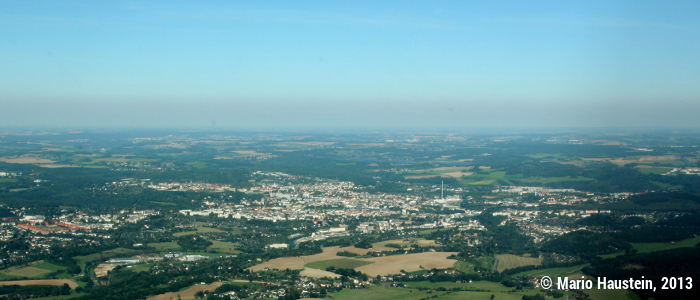
\includegraphics[width=\hsize]{bilder/titelbild}}

\setbeamertemplate{title page}[tucpicture]
\frame{\maketitle}
\endgroup
\end{lstlisting}
\endgroup

\bigskip

\item Anstatt \texttt{tucpicture} kann auch \texttt{tucnarrowpicture} angegeben werden.
  \begin{itemize}
  \item Das Titelbild erstreckt sich dann ggf. \structure{nicht} über die Logo-Spalte.
  \item Dies muss natürlich beim Seitverhältnis des Titelbilds berücksichtigt werden.
  \end{itemize}
\end{itemize}
\end{frame}


\tucthreeheadlines
\begingroup
\title{Demo-Titel}
\titlegraphic{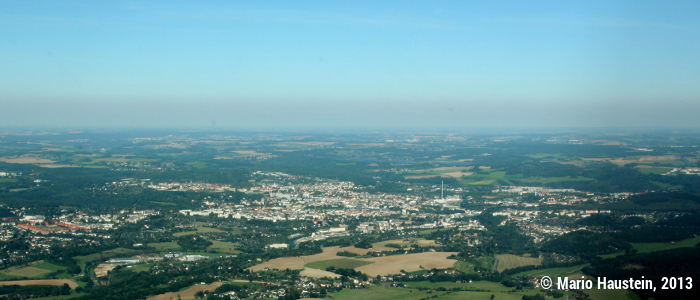
\includegraphics[width=\hsize]{bilder/titelbild}}

\setbeamertemplate{title page}[tucpicture]
\frame{\maketitle}
\endgroup
\tuctwoheadlines


\subsection{Das \LaTeX-Beamer-Grundgerüst}
\begingroup
\newcommand{\mymark}[1]{\hspace*{4em}\llap{\texttt{#1}}}

\begin{frame}
\frametitle{Verzeichnisstruktur der Vorlage}

\begin{itemize}
\item Neben dem Makefile enthält die Vorlage eine Reihe von \TeX-Dateien.
\item Der eigentliche Inhalt der Präsentation wird in \texttt{main.tex} kodiert.
\item Zusätzlich existieren die folgenden Dateien, die ihrerseits \texttt{main.tex} einbinden.
  \begin{description}
  \item[\mymark{beamer.tex}]  Erstellt die Präsentation zur Anzeige auf einem Beamer.
  \item[\mymark{dualmon.tex}] Erstellt ein PDF doppelter Breite. Die linke
                              Hälfte enthält die eigentliche Beamer-Präsentation.
                              Die rechte Hälfte die Anmerkungen zur Anzeige auf dem
                              Laptop-Bildschirm.
  \item[\mymark{notes.tex}]   Druckversion der Präsentation mit Anmerkungen.
  \item[\mymark{handout.tex}] Druckversion der Präsentation zur Veröffentlichung.
  \end{description}
\end{itemize}
\end{frame}
\endgroup

\begin{frame}
\frametitle{Overlays}

\begin{itemize}
\item Die Overlays funktionieren wie gewohnt. Für eine detaillierte Einführung siehe~\cite{beamerguide}.
\bigskip
\item Das vorliegende Grundgerüst nutzt die Modi \texttt{beamer}, \texttt{handout} und \texttt{trans}.
\item Die Modi können benutzt werden, um abweichende Ausgaben für die Notizen oder die Druckversion zu erzielen.
  \begin{description}
  \item[\texttt{beamer}]  Wird für die Erstellung der eigentlichen Beamerpräsentation
                          genutzt (auch für die Version mit zwei Bildschirmen).
  \item[\texttt{handout}] Wird für die Druckversion genutzt. "`Aufblättereffekte"'
                          sollten folglich vermieden werden. Weiterhin kann ergänzendes
			  Zusatzmaterial eingebunden werden.
  \item[\texttt{trans}]   Wird für die Referentennotizen genutzt und dient im
                          wesentlichen dazu, die "`Aufblättereffekte"' sinnvoll
			  zusammenzufassen.
  \end{description}
\end{itemize}
\end{frame}



\section{Verschiedenes}
\subsection{Kontakt}
\begin{frame}
\frametitle{Fragen, Anmerkungen, Wünsche, Bugs \dots}
\framesubtitle{\dots\ nimmt entgegen \dots}

\begin{center}
\scalebox{1.5}{\url{mario.haustein@hrz.tu-chemnitz.de}}
\end{center}
\end{frame}


\subsection{Literatur}
\begin{frame}
\frametitle{Literatur}

Ich empfehle unbedingt \dots

\bigskip

\begin{thebibliography}{xxx}
\bibitem{beamerguide} The Beamer class
\newblock{\url{http://www.ctan.org/tex-archive/macros/latex/contrib/beamer/doc/beameruserguide.pdf}}
\end{thebibliography}
\end{frame}



\section{}
\frame<beamer| trans>{\Huge\begin{center}\scalebox{2}{\texttt{\textbackslash endinput}}\end{center}}

\end{document}
